\chapter{Explicit One-Step Methods and Convergence}

\section{Introduction}
\begin{example}[Euler's method]
  We begin this section with the method which serves as prototype for
  a whole class of schemes which solves an IVP or rather the Volterra
  integral equation numerically. Here, as always for problems with
  infinite dimensional solution spaces, numerical solution refers to
  finding an approximation by applying a discretization method, and
  studying the error of this method.
  
  Consider the following problem: given an IVP of the form~\eqref{eq:awa},
  calculate the value $u(T)$ at a later point in time $T$.
  
  To this end, we note first of all that for an IVP at the initial
  point $0$, not only the function value $u(0) = u_0$ is known,
  but also the derivative $u'(0) = f(0, u_0)$. Thus we are capable
  to replace the solution $u(t)$ in blue by a straight line $y(t)$ in
  red, which we can see on the left of Figure~\ref{fig:explicit:Euler}.
  \begin{figure}[tp]
    \centering
    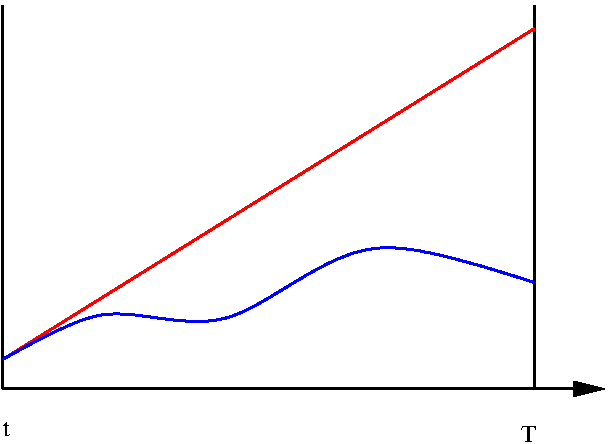
\includegraphics[width=.48\textwidth]{fig/euler1}
    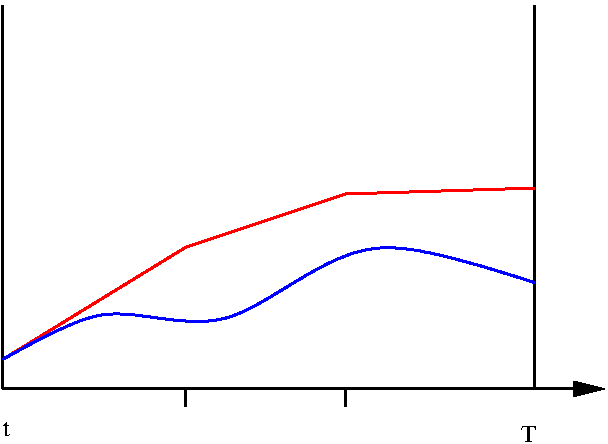
\includegraphics[width=.48\textwidth]{fig/euler2}
    \caption{Derivation of the Euler method. Left: replacement of the
			solution of the IVP by a line with slope and initial point given 
			by the IVP. Right: Euler method with three subintervals.}
    \label{fig:explicit:Euler}
  \end{figure}
  The figure suggests that in general the accuracy of this method may
  not be very good. The first improvement is that we do not draw the
  line through the whole interval from $0$ to $T$.  Instead, we
  insert intermediate points and apply the method to each subinterval,
  where we use the result of a previous interval as the initial point
  for the next subinterval.  As a result one obtains a
  chain of straight lines and the so-called \define{Euler method}.
\end{example}


\begin{Definition}{partitioning}
  On a time interval $I = [0,T]$, we define a partitioning in $n$
  subintervals, also known as \textbf{time steps}.\defindex{time step}
  Here we choose the following notation:
%  \begin{figure}[tp]
  \begin{center}
    \small
    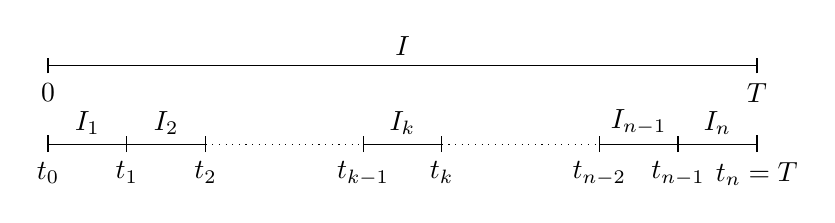
\begin{tikzpicture}
      \draw(0,1) -- node [anchor=south]{$I$} (9,1);
      \draw[thick](0,.9) node[anchor=north]{$0$} -- (0,1.1);
      \draw[thick](9,.9) node[anchor=north]{$T$} --(9,1.1);

      \draw(0,0)-- node [anchor=south]{$I_1$}(1,0);
      \draw(1,0)-- node [anchor=south]{$I_2$}(2,0);
      \draw(4,0)-- node [anchor=south]{$I_k$}(5,0);
      \draw(7,0)-- node [anchor=south]{$I_{n-1}$}(8,0);
      \draw(8,0)-- node [anchor=south]{$I_{n}$}(9,0);
      \draw[dotted](2,0)--(4,0);
      \draw[dotted](5,0)--(7,0);
      \draw[thick](0,-.1) node[anchor=north]{$t_0$} -- (0,.12);
      \draw(1,-.1) node[anchor=north]{$t_1$} --(1,.1);
      \draw(2,-.1) node[anchor=north]{$t_2$} --(2,.1);
      \draw(4,-.1) node[anchor=north]{$t_{k-1}$} --(4,.1);
      \draw(5,-.1) node[anchor=north]{$t_k$} --(5,.1);
      \draw(7,-.1) node[anchor=north]{$t_{n-2}$} --(7,.1);
      \draw(8,-.1) node[anchor=north]{$t_{n-1}$} --(8,.1);
      \draw[thick](9,-.1) node[anchor=north]{$t_n=T$} --(9,.12);
    \end{tikzpicture}
  \end{center}
%    \caption{Partition of the interval $I=[0,T]$ in subintervals $I_1,\dots,I_n$.}
%    \label{fig:explicit:schritte}
%  \end{figure}
  The time steps $I_k = [t_{k-1},t_{k}]$ have the step size
  $h_k = t_{k} - t_{k-1}$.  A partitioning in $n$ time steps implies
  $t_n = T$.  The term $k$-th time step is used for both the interval
  $I_k$ and for the point in time $t_k$, but it should always be clear
  through context which one is meant.

  Very often, we will consider evenly spaced time steps, in which case
  we denote the step size by $h$ and $h_k=h$ for all $k$.
\end{Definition}

%%% Local Variables:
%%% mode: latex
%%% TeX-master: "../notes"
%%% End:


\begin{definition}
  In the following chapters we will regularly compare the solution of
  an IVP with the results of discretization methods. Therefore, we
  introduce the following convention for notations and symbols.
  
  \defindex{solution!continuous}\defindex{solution!exact} The solution
  of the IVP is called the \textbf{exact} or \define{continuous
    solution}\defindex{exact solution}. The term ``continuous''
  indicates here the solution of the non-discretized problem. Its
  symbol is in general $u$ and we set as abbreviation
  \begin{gather*}
    u_k = u(t_k).
  \end{gather*}
  If $u$ is vector-valued we also use the alternative superscript
  $u^{(k)}$ and $u_i^{(k)}$ for a entry of the vector $u(t_k)$.

  \defindex{solution!discrete} In general we write the
  \define{discrete solution} with the
  symbol $y$. We write $y_k$ or $y^{(k)}$ for the value of the
  discrete solution at the point in time $t_k$. In contrast to the
  continuous solution, $y$ only defined at discrete time steps, unless
  for special methods discussed later.
\end{definition}

\begin{Definition*}{one-step}{Explicit one-step method}
  \defindex{One-step method!explicit} An \textbf{explicit one-step
    method} \defindex{Explicit one-step method} is a method which,
  given $u_0$ at $t_0 = 0$ computes a sequence of approximations
  $y_1\,\dots,y_n$ to the solution of an IVP in the time steps
  $t_1,\dots,t_n$ using an update formula of the form\footnote{The adjective
  `explicit' is here in contrast to `implicit'
  one-step methods, where the increment function depends 
	on $y_{k}$ and equation~\eqref{eq:explicit:8} must be solved
        for $y_{k}$.}
  \begin{gather}
    \label{eq:explicit:8}
    y_{k} = y_{k-1} + h_{k} \verfahren_{h_k}(t_{k-1},y_{k-1}).
  \end{gather}
  The function $\verfahren()_{h_k}$ is called \define{increment
    function}.  We will often omit the index $h_k$ on
  $\verfahren_{h_k}()$ because it is clear that the method is always
  applied to time intervals.

  The method is called \textbf{one-step method}
  because the value $y_{k}$ explicitly depends only of the values
  $y_{k-1}$ and $f(t_{k-1}, y_{k-1})$, not on previous values.
\end{Definition*}

%%% Local Variables:
%%% mode: latex
%%% TeX-master: "../notes"
%%% End:


\begin{remark}
  \label{remark:expl:first-step}
  For one-step methods every step is \emph{per definitionem} similar.
  Therefore, it is sufficient to consider the first step only.  Hence,
  we will define and analyze methods by stating the dependence of
  $y_1$ on $y_0$ which then can be transferred to the general step
  from $y_{n-1}$ to $y_{n}$. The general one-step method above then
  reduces to
  \begin{gather*}
    y_1 = y_0 + h \verfahren(t_0, y_0).
  \end{gather*}
  This implies that the values $y_k$ with $k\ge 2$ are computed
  through formula~\eqref{eq:explicit:8} with the respective $h_k$ and
  the same increment function.
\end{remark}

\begin{Example}{euler-linear-1}
  Given the IVP
  \begin{xalignat*}2
    u'  &= u,&
    u(0) &= 1,    
  \end{xalignat*}  
  the solution is $u(t) = e^t$. The Euler method reads
  \begin{gather*}
    y_1 = y_0 + h y_0.
  \end{gather*}
  The results for $h=1$ and $h=1/2$ are:
  \begin{center}
    \begin{tabular}{cc|ccc|ccc}
      \multicolumn{2}{c|}{exact}
      &\multicolumn{3}{c|}{$h=1$}
      &\multicolumn{3}{c}{$h=1/2$}\\\hline
      $t=0$ & 1           & $y_0$ & 1     && $y_0$ & 1 & \\
      $t=1$ & 2.71828     & $y_1$ & 2     & 0.718 & $y_2$ & 2.25  & 0.468\\
      $t=2$ & 7.38906     & $y_2$ & 4     & 3.389 & $y_4$ & 5.0625& 2.236\\\hline
      $t=k$ & $2.71828^k$ & $y_k$ & $2^k$ && $y_{2k}$ & $2.25^k$
    \end{tabular}    
  \end{center}
  We note that the error is growing in time. The approximation of the
  solution can be improved by shrinking $h$ from 1 to 1/2. The goal of
  error analysis will be establishing these dependencies.
\end{Example}

%%% Local Variables:
%%% mode: latex
%%% TeX-master: "../notes"
%%% End:


%%%%%%%%%%%%%%%%%%%%%%%%%%%%%%%%%%%%%%%%%%%%%%%%%%%%%%%%%%%%%%%%%%%%%%
%%%%%%%%%%%%%%%%%%%%%%%%%%%%%%%%%%%%%%%%%%%%%%%%%%%%%%%%%%%%%%%%%%%%%%
\section{Error analysis}
%%%%%%%%%%%%%%%%%%%%%%%%%%%%%%%%%%%%%%%%%%%%%%%%%%%%%%%%%%%%%%%%%%%%%%
%%%%%%%%%%%%%%%%%%%%%%%%%%%%%%%%%%%%%%%%%%%%%%%%%%%%%%%%%%%%%%%%%%%%%%

\begin{remark}
  In Figure~\ref{fig:explicit:Euler}, we observe that the error
  consists of two parts at a given time $t_{k+1}$. First, an error on
  the interval $I_k$ due to replacing the differential equation by the
  discrete method. Second, we have to add the error which results from
  the fact that our initial value $y_k$ is already not exact due to
  previous errors. This situation is displayed in
  Figure~\ref{fig:forward-errors}. After one time step, a local error
  has appeared. In the second time step, we already start with an
  erroneous initial value. Therefore, we split the error into the
  local error and an accumulated error. The local error compares
  continuous and discrete solutions on a single interval with the same
  initial value. In the analysis, we will have the options of using
  the exact (right figure) or the approximated initial value (left figure).

  \begin{figure}[tp]
    \centering
    \includegraphics[width=.49\textwidth]{fig/forward-error.tikz}
    \includegraphics[width=.49\textwidth]{fig/backward-error.tikz}
    \caption{Local and accumulated errors. Exact solution in black,
      the Euler method in red. On the left, in blue the exact solution
      of an IVP on the second interval with initial value $y_1$. On
      the right, in purple the second step of the Euler method, but with
      exact initial value $u_1$.}
    \label{fig:forward-errors}
  \end{figure}
\end{remark}

\begin{Definition}{truncation-error}
  Let $u$ be a solution of the differential equation $u' = f(t,u)$
  on the interval $I_n = [t_{n-1}, t_{n}]$. Then, the \define{local
    error} of a discrete method $F$ is the difference between the
  solution $u_n$ of the differential equation at $t_n$ and the result
  of one time step~\eqref{eq:explicit:8} with this method with exact
  initial value:
  \begin{gather}
    \label{eq:explicit:6a}
    \eta_{n} = \eta_n(u) = u_{n} - \bigl[
    u_{n-1} + h_n \verfahren_{h_n}(t_{n-1}, u_{n-1})
    \bigr].
  \end{gather}
  The \define{truncation error} is the quotient of the local error and $h_n$:
  \begin{gather}
    \label{eq:explicit:6}
    \tau_{n} = \tau_n(u) = \frac{u_{n} - u_{n-1}}{h_n} - \verfahren_{h_n}(t_{n-1}, u_{n-1}).
  \end{gather}
  \defindex{order!of consistency}
  The one-step method $F_h(t,y)$ is \define{consistent} of \textbf{order} $p$ with
  the ODE, if there is a constant $c$ independent of $h$ such that for
  $h\to 0$:
  \begin{gather}
    \label{eq:explicit:3}
    \max\limits_n \abs{\tau_n} \le c h^p
  \end{gather}
\end{Definition}

%%% Local Variables:
%%% mode: latex
%%% TeX-master: "../notes"
%%% End:


\begin{example}[Euler method]
  To find out the order of consistency of the Euler method, we 
  consider the Taylor expansion of the solution at the point $t_{n-1}$:
  \begin{equation*}
    u(t_n) = u(t_{n-1}) + h_n u'(t_{n-1}) + \frac12 h_n^2 u''(\zeta)
  \end{equation*}
  
  As a result the truncation error reduces to:
  
  \begin{align*}
    \tau_n & = \frac{u_n - u_{n-1}}{h_n} - F(h;t_{n-1},u(t_{n-1})) \\
    & = \frac{u_{n-1} + h_n f(t_{n-1},u_{n-1})
      + \frac12 h_n^2 u''(\zeta) - u_{n-1}}{h_n} - f(t_{n-1}; u_{n-1}) \\
    & = \frac12 h_n u''(\zeta)
  \end{align*}

% For $u''(\zeta)$ however there holds:
% \begin{equation*}
%   u''(\zeta) = \diffq[\zeta] f(\zeta,u(\zeta)) = \pdiffq[\zeta] f(\zeta,u(\zeta)) + \pdiffq[u] f(\zeta,u(\zeta)) \underbrace{u'(\zeta)}_{= f(\zeta,u(\zeta))}
% \end{equation*}

Under the assumption that $f \in C^1$ on a compact set around the graph
of $u$, this term is bounded, yielding.
\begin{gather*}
  | \tau_n | \le \frac{h_n}{2} \max_{\zeta\in I_n} \abs{u''(\zeta)}
  = \frac{h_n}{2} \max_{\zeta\in I_n} \bigl|\partial_x f(\zeta,
    u(\zeta)) + \partial_u  f(\zeta, u(\zeta)) f(\zeta, u(\zeta))\bigr|
\end{gather*}
Here, we enter the assumption that $f$ is sufficiently smooth to
conclude that the Euler method is consistent of order 1.
\end{example}

\begin{Lemma*}{gronwall-discrete}{Discrete Grönwall inequality}
  \index{Grönwall's inequality} Let $(w_n)$, $(a_n)$ and $(b_n)$ be
  non-negative sequences of real numbers. Let $b_n$ be monotonically
  nondecreasing. Then, if
  \begin{gather}
    \label{eq:gronwall-discrete:1}
    w_0 \le b_0
    \quad\text{and}\quad
    \forall n\ge 1 :\;
    w_n \le \sum\limits_{k=0}^{n-1} a_k w_k + b_n,
  \end{gather}
  there holds
  \begin{gather}
    \label{eq:explicit:5}
    w_n \le \exp \left(\sum\limits_{k=1}^{n-1} a_k\right) b_n.
  \end{gather}
\end{Lemma*}

%%% Local Variables:
%%% mode: latex
%%% TeX-master: "../notes"
%%% End:


\begin{proof}
  Define the functions $w(t)$, $a(t)$, and $b(t)$ such that for $k\ge
  1$ and $t\in [k-1,k)$ there holds
  \begin{gather*}
    w(t) = w(t_{k-1}),\quad
    a(t) = b(t_{k-1}),\quad
    b(t) = b(t_{k-1}).
  \end{gather*}
  These functions are bounded and piecewise continuous on any finite
  interval. Thus, they are integrable on $[0,n]$. Therefore, the
  continuous Grönwall inequality of Lemma~\ref{Lemma:gronwall} applies
  and proves the result.
\end{proof}

\begin{Theorem*}{stability-discrete}{Discrete stability}
  If $F(t,y)$ is Lipschitz continuous in $y$ for any $t=t_k$, $k<n$,
  with constant $L_h$, then the one-step method is \define{discretely
    stable}, i.~e. for arbitrary sequences $(y_n)$ and $(z_n)$, there
  holds: if $\eta_k(y)$ and $\eta_k(z)$ are both bounded independent
  of the sequences $(y_n)$ and $(z_n)$, then
  \begin{equation*}
    \abs{y_n - z_n}
    \le e^{L_h(t_n-t_0)} \left(
      \abs{y_0 - z_0}
      + \sum_{k=1}^n \abs{\eta_k(y) - \eta_k(z)}
    \right)
  \end{equation*}
\end{Theorem*}

%%% Local Variables:
%%% mode: latex
%%% TeX-master: "../notes"
%%% End:


\begin{proof}
  Subtracting the equations
  \begin{align*}
    \eta_k(y) &= y_k-y_{k-1} - \verfahren_{h_k}(t_{k-1},y_{k-1}),
    \\
    \eta_k(y) &= z_k-z_{k-1} - \verfahren_{h_k}(t_{k-1},z_{k-1}),
  \end{align*}
  we obtain
  \begin{multline*}
    y_k-z_k = y_{k-1} - z_{k-1} + \eta_k(y) - \eta_k(z)
    \\
    + h_k \bigl(
      F_{h_k}(t_{k-1},y_{k-1})-F_{h_k}(t_{k-1},z_{k-1})
    \bigr)
    .
  \end{multline*}
  Recursive application yields
  \begin{gather*}
    \abs{y_n-z_n} \le \abs{y_0-z_0}
    + \sum_{k=1}^n \abs{\eta_k(y)-\eta_k(z)}
    + \sum_{k=1}^n L_h h_{k} \abs{y_k-z_k}.
  \end{gather*}
  The estimate now follows from the discrete Grönwall inequality in
  Lemma~\ref{Lemma:gronwall-discrete}.
\end{proof}

\begin{Corollary*}{finite-precision}{One-step methods with finite precision}
  Let the one-step method $\verfahren$ be run on a computer, yielding
  a sequence $(z_n)$, such that each time step is executed in finite
  precision arithmetic. Let $(y_n)$ be the mathematically correct
  solution of the one-step method. Then, the difference
  equation~\eqref{eq:explicit:8} is fulfilled only up to machine
  accuracy $\epsilon_m$:
  \begin{align*}
    y_0-z_0 &\approx \epsilon_m \\
    \abs{\eta_k(y) - \eta_k(z)} &= \abs{\eta_k(z)} \approx \epsilon_m \abs{z_k}.
  \end{align*}
  Then, the error between the true solution of the one-step method
  $(y_n)$ and the computed solution is bounded by
  \begin{gather*}
    \abs{y_n-z_n} \le e^{L_h(t_n-t_0)} n \epsilon_m \max_k\abs{z_k}.
  \end{gather*}
\end{Corollary*}

\begin{Theorem*}{convergence-one-step}{Convergence of one-step methods}
  Let the one-step method $F(.,.)$ be consistent of order $p$ and
  discretely stable, that is, $F(.,.)$ is Lipschitz continuous in its
  second argument. Let $f(t,u)\in C^{p}$. Furthermore, let be
  $y_0 = u_0$. Let $h = \max h_n$ and let there be a positive number
  $\gamma$ such that $\min h_n = \gamma h$. Then, the method converges
  with order $p$ and there holds for
  \begin{equation}
    \label{eq:convergence-onestep:1}
    \abs{u_n - y_n} \le c e^{L_h(t_n-t_0)} h^p,
  \end{equation}
  where the constant $c$ is independent of $h$.
\end{Theorem*}

\begin{proof}
  Again we use the discrete stability theorem: with the definition of
  the order of the method, we obtain
  \begin{gather}
    \label{eq:convergence-onestep:2}
    \abs{\eta_k(u)-\eta_k(y)} = \abs{\eta_k(u)} \le c h^{p+1},
  \end{gather}
  where $c$ depends on the derivatives of $u$ (and thus of $f$), but
  not on $u_k-y_k$. On the other hand, we have
  \begin{gather*}
    n \le \frac{t_n-t_0}{\min h_n} \le \frac{t_n-t_0}{\gamma h}.
  \end{gather*}
  Thus, we obtain by summing up~\eqref{eq:convergence-onestep:2} over all $n$
  \begin{gather*}
    \abs{u_n-y_n} \le e^{L_h(t_n-t_0)}\sum_{k=1}^n h_k^{p+1}
    \le c e^{L_h(t_n-t_0)} h^p.
  \end{gather*}
\end{proof}

\begin{corollary}
  The Euler method converges of first order.
\end{corollary}

%%%%%%%%%%%%%%%%%%%%%%%%%%%%%%%%%%%%%%%%%%%%%%%%%%%%%%%%%%%%%%%%%%%%%%
%%%%%%%%%%%%%%%%%%%%%%%%%%%%%%%%%%%%%%%%%%%%%%%%%%%%%%%%%%%%%%%%%%%%%%
\section{Runge-Kutta methods}
%%%%%%%%%%%%%%%%%%%%%%%%%%%%%%%%%%%%%%%%%%%%%%%%%%%%%%%%%%%%%%%%%%%%%%
%%%%%%%%%%%%%%%%%%%%%%%%%%%%%%%%%%%%%%%%%%%%%%%%%%%%%%%%%%%%%%%%%%%%%%

\begin{intro}
  We are searching for methods which approximate the solution to an
  IVP numerically.  In fact we are not solving the IVP, but the Volterra
  integral equation~\eqref{eq:volterra}.  Hence we can consider
  solving differential equations as a quadrature problem; with the
  difficulty that the function, which we integrate, is not known. This
  consideration leads to a class of methods for IVP, the
  Runge-Kutta methods.
\end{intro}

\begin{Definition}{erk}
  \defindex{Runge-Kutta method!explicit (ERK)}
  \index{ERK|see{Runge-Kutta method}} 
  An \textbf{explicit Runge-Kutta method (ERK)} is a
  one-step method with the representation
  \begin{subequations}
    \label{eq:explicit:1}
    \begin{xalignat}{2}
      \label{eq:explicit:1a}
      \rkg_i &= y_0 + h \sum_{j=1}^{i-1} \rka_{ij} k_j
      & i &= 1,\dots,\rks
      \\
      \label{eq:explicit:1b}
      k_i &= f\left(h \rkc_i, \rkg_i\right)
      & i &= 1,\dots,\rks
      \\
      \label{eq:explicit:1c}
      y_1 &= y_0 + h \sum_{i=1}^{\rks} \rkb_i k_i
    \end{xalignat}
  \end{subequations}
  In this method the values $h\rkc_i$ are the quadrature points
  on the interval $[0,h]$. The values $k_i$ are approximations to
  function values of the integrand in these points and the values $\rkg_i$ constitute
  approximations to the solution $u(h\rkc_i)$ in the quadrature
  points. This method uses $s$ intermediate values and is thus called
  an $\rks$-stage method.
\end{Definition}

%%% Local Variables:
%%% mode: latex
%%% TeX-master: "../notes"
%%% End:


\begin{remark}
  Pursuant to remark~\ref{remark:expl:first-step} we present the
  formula for the calculation of $y_1$ from $y_0$ on the interval from
  $t_0=0$ to $t_1 = h$.  The formula for a later time step $k$ is
  obtained by replacing $y_0$ and $t_0=0$ by $y_k$ and $t_k$,
  respectively to obtain $y_{k+1}$.
\end{remark}

\begin{remark}
  The intermediate values $\rkg_i$ will not be saved separately in
  typical implementations, because it is possible to execute the
  method with the values $k_i$ alone. Nevertheless, the values
  $\rkg_i$ are useful for highlighting the structure of the method.
\end{remark}

\begin{Definition*}{butcher-tableau-erk}{Butcher tableau}
  It is customary to write Runge-Kutta methods in the form of a
  \define{Butcher tableau}, containing only the coefficients of
  equation~\eqref{eq:explicit:1} in the following matrix form:
\begin{gather}
  \label{eq:explicit:2}
  \begin{array}{c|ccccc}
    0 & \\
    \rkc_2 & \rka_{21} \\
    \rkc_3 & \rka_{31} & \rka_{32} \\
    \vdots & \vdots & \vdots & \ddots \\
    \rkc_\rks & \rka_{\rks1} & \rka_{\rks2} & \cdots & \rka_{\rks,\rks-1} \\
    \hline
    & \rkb_1 & \rkb_2 & \cdots & \rkb_{\rks-1} & \rkb_\rks \\
  \end{array}
\end{gather}
\end{Definition*}

%%% Local Variables:
%%% mode: latex
%%% TeX-master: "../notes"
%%% End:


\begin{remark}
  The first row of the tableau is to read in such a manner, that
  $g_1 = y_0$ and $k_1$ is computed directly by $f(t_0, y_0)$. The
  coefficients $a_{1j}$ and $c_0$ do not appear in formulas~\eqref{eq:explicit:1a}
  and~\eqref{eq:explicit:1b} (or are considered zero).
  
  The further rows indicate the rules for the computation of the
  further values $k_i$ in each case according to the
  formulas~\eqref{eq:explicit:1a} and~\eqref{eq:explicit:1b}. The
  the method is explicit since the computation of $k_i$ only involves
  coefficients with index less than $i$.
  
  The last row below the line is then the short form of
  formula~\eqref{eq:explicit:1c} and lists quadrature weights.

  We see, that the coefficients $a_{ij}$ form the strict lower
  triangle of a square $s\times s$-matrix $A$. Therefore, in order to
  simplify the summation bounds, we implicitly complete this matrix
  with values $a_{ij} = 0$ for $j\ge i$.This way, the sum
  in~\eqref{eq:explicit:1a} can be taken from $1$ to $s$, independent
  of $i$. We will also associate to an $s$-stage method the vector $b
  = (b_1,\dots,b_s)^T$.
\end{remark}

\begin{example}
  The Euler method \putindex{Euler method} has the \putindex{Butcher
    tableau}:
  \begin{gather*}
    \begin{array}{c|c}
      0 & \\
      \hline
        & 1 \\
    \end{array}
  \end{gather*}
  That leads to the already known formula:
  \begin{equation*}
    y_1 = y_0 + h f(t_0, y_0)
  \end{equation*}
  The values $b_1=1$ and $c_1=0$ indicate that this is a quadrature
  rule with a single point at the left end of the interval. Such a
  rule is exact for constant polynomials and thus of order 1.
\end{example}

\begin{Example*}{rk2}{Two-stage methods}
  \index{Euler method!modified} The \define{modified Euler method} is
  a variation of the Euler method of the following form:
  \begin{gather*}
    \begin{aligned}
      k_1 & = f(t_0,y_0) \\
      k_2 & = f(t_0 + \frac12 h, y_0 + h \frac12 k_1) \\
      y_{1} & = y_0 + h k_2
    \end{aligned}
    \qquad
    \begin{array}{c|cc}
      0 & \\
      \frac12 & \frac12 \\
      \hline
        & 0 & 1
    \end{array}
  \end{gather*}

  The so-called \define{Heun method} of order 2 is characterized
  through the equation
  \begin{gather*}
    \begin{aligned}
      k_1 & = f(t_0, y_0) \\
      k_2 & = f(t_0 + h, y_0 + h k_1) \\
      y_{1} & = y_0 + h ( \frac12 k_1 + \frac12 k_2 ) \\
    \end{aligned}
    \qquad
    \begin{array}{c|cc}
      0 & \\
      1 & 1 \\
      \hline
        & \frac12 & \frac12 \\
    \end{array}
  \end{gather*}
\end{Example*}

%%% Local Variables: 
%%% mode: latex
%%% TeX-master: "../notes"
%%% End: 


\begin{remark}
  The modified Euler method uses an approximation to the value of
  $f(h/2, u(h/2))$ in its quadrature, corresponding to the midpoint
  quadrature rule. The Heun method is constructed analogous to the
  trapezoidal rule. Both quadrature rules are of second order, and so
  are these one-step methods.  Both methods were discussed by Runge in
  his article of 1895~\cite{Runge95}.
\end{remark}

\begin{Lemma}{Heun-consistency}
  The Heun method and the modified Euler method are consistent of second
  order\footnote{Here and in the following proofs of consistency
    order, we will always assume that all necessary derivatives of $f$
  exist and are bounded. We say ``$f$ is sufficiently smooth''.}.
\end{Lemma}

\begin{proof}
  The proof uses Taylor expansion of the continuous solution $u$ and
  the discrete solution $y$ around $t_0$ with respect to $h$. First,
  abbreviating $f_t = \partial_t f(t_0,u_0)$ and
  $f_u = \partial_u f(t_0,u_0)$ and so forth\footnote{Note that $f_u$,
    $f_{u u}$ and so on are tensors of increasing rank.} and replacing
  $u'(t_0)=f(t_0,u_0) = f$:
  \begin{multline}
    \label{eq:explicit:4}
    u_1 = u(t_0+h) = u_0 + h f(t_0, u_0)
    + \frac{h^2}2\bigl(f_t + f_u f\bigr)
    \\
    + \frac{h^3}6\bigl(f_{t t}+2f_{t u}f+f_{u u}f^2+f_u f_t+f_u^2f\bigr)
    + \dots.
  \end{multline}
  For the discrete solution of the modified Euler step on the other
  hand, there holds
  \begin{align*}
    y_1 &= u_0 + h f\left(t_0+\frac h2, u_0+\frac h2 f(t_0,u_0)\right)
    \\
    &= u_0 + h f(t_0, u_0) + \frac{h^2}2 \bigl(f_t + f_u f\bigr)
    \\&\hphantom{...}
      + \frac{h^3}8\bigl(f_{t t}+2f_{t u}f+f_{u u}f^2+f_u f_t+f_u^2f\bigr)
        +\dots.
  \end{align*}
  Thus, $\abs{u_1-y_1} = \mathcal O(h^3)$ and the method is of second
  order. The proof for the Heun method is left as an exercise.
\end{proof}

\begin{Example}{rk3}
  \defindex{Runge-Kutta method!three-stage}
  The three stage Runge-Kutta method is

  \begin{gather*}
    \begin{aligned}
      k_1 & = f(t_0, y_0) \\
      k_2 & = f(t_0 + \frac12 h, y_0 + \frac12 h k_1) \\
      k_3 & = f(t_0 + h, y_0 - h k_1 + 2 h k_2) \\
      y_{n+1} & = y_0 + h ( \frac16 k_1 + \frac46 k_2 + \frac16 k_3 ) \\
    \end{aligned}
    \qquad
    \begin{array}{c|ccc}
      0 & \\
      \frac12 & \frac12 \\
      1 & -1 & 2 \\
      \hline
        & \frac16 & \frac46 & \frac16 \\
    \end{array}
  \end{gather*}
  This method is obviously based on the Simpson rule.
\end{Example}

\begin{remark}
  Computations become tedious very fast, in part due to the sum of
  partial derivatives of $f(t,u)$. This can be simplified by
  considering Runge-Kutta methods for the autonomized ODE (see
  Definition~\ref{Definition:autonomization})
  \begin{gather*}
    \begin{pmatrix} u' \\ t' \end{pmatrix} = 
    \begin{pmatrix} f(t,u) \\ 1 \end{pmatrix}.
  \end{gather*}
  Then,the Runge-Kutta method~\eqref{eq:explicit:1} simplifies to
  \begin{gather}
    \label{eq:explicit:7a}
    \begin{split}
      \rkg_i &= y_0 +
      \sum_{j=1}^{i-1} \rka_{ij} h f(\rkg_j),\quad i=1,\dots,\rks
      \\
      y_1 &= y_0 + \sum_{j=1}^s b_j h f(g_j).
    \end{split}
  \end{gather}
\end{remark}

\begin{Lemma}{erk-autonomization}
  An ERK is invariant under autonomization (or in short,
  \putindex{autonomizable}), if and only if
  \begin{gather}
    \label{eq:explicit:9}
    c_i = \sum_{j=1}^{i-1} a_{ij}, \quad i=1,\dots,s.
  \end{gather}
\end{Lemma}

\begin{proof}
  Observing the last component of the vector $u$ in the previous
  remark and the method applied to it yields the condition.
\end{proof}

%HNW p. 145 and pp. 135/137
\begin{Lemma}{rk-order-3-4}
  An autonomizable ERK with $s$ stages is consistent of third order, if
  and only if the following conditions are met:
  \begin{subequations}
    \label{eq:explicit:11}
    \begin{align}
      \label{eq:explicit:12}
      b_1 + \dots + b_s &= 1, \\
      \label{eq:explicit:13}
      b_1c_1 + \dots + b_s c_s &= 1/2, \\
      \label{eq:explicit:14}
      b_1c_1^2 + \dots + b_s c_s^2 &= 1/3, \\
      \label{eq:explicit:15}
      \sum\nolimits_{i,j} b_i a_{ij}c_j &= 1/6.
    \end{align}
    It is consistent of fourth order, if and only if additionally
    \begin{align}
    \label{eq:explicit:16}
    b_1c_1^3 + \dots + b_s c_s^3 &= 1/4, \\
    \label{eq:explicit:18}
    \sum\nolimits_{i,j} b_i a_{ij} c_j^2 &= 1/12, \\
    \label{eq:explicit:19}
    \sum\nolimits_{i,j,k} b_i a_{ij} a_{jk} c_k &= 1/24,\\
    \label{eq:explicit:17}
    \sum\nolimits_{i,j} b_i c_i a_{ij} c_j &= 1/8.
  \end{align}
  \end{subequations}
\end{Lemma}

\begin{remark}
  We can rephrase these conditions, such that an ERK is of order $k$ if
  the quadrature with
  support points $c_i$ and corresponding weights $b_i$ is exact for
  polynomials of degree $k-1$:
  \begin{gather*}
    \sum_{i=1}^{s} b_i p(c_i) = \int_0^1 p(t)\dt,
    \qquad \forall p\in \P_{k-1}.
  \end{gather*}
  Furthermore, for $k \ge 3$
  \begin{gather*}
    \sum_{ij} b_i a_{ij} p(c_j) = \int_0^1\int_0^t p(s)\ds\dt,
    \qquad \forall p\in \P_{k-2}.
  \end{gather*}
  Additionally, for $k\ge 4$
  \begin{xalignat*}2
    \sum_{ijk} b_i a_{ij} a_{jk} p(c_k) &= \int_0^1\int_0^t\int_0^s p(r)\dr \ds \dt,
    &&\forall p\in \P_{k-3},\\
    \sum_{ij} b_i p(c_i) a_{ij} q(c_j)
    &= \int_0^1 p(t) \int_0^t q(s) \ds\dt
    &&\forall p\in \P_{k_1}, q\in\P_{k_2}, k_1+k_2 = k-2.
  \end{xalignat*}
\end{remark}

\begin{Lemma}{taylor-u}
  The Taylor expansion of a single component of $u_1 = u(h)$ with
  respect to $h$ is
  \begin{gather}
    \label{eq:taylor-u:1}
    \begin{split}
      (u_1)_n &= (u_0)_n
      \\& + h f_n
      \\& + \frac{h^2}2 \sum_\lambda \partial_{\lambda} f_n f_\lambda
      \\& + \frac{h^3}6 \sum_{\lambda,\mu} \bigl[\partial_{\lambda\mu} f_n f_\lambda f_\mu
      + \partial_{\lambda}f_n \partial_{\mu}f_\lambda f_\mu\bigr]
      \\& + \frac{h^4}{24} \sum_{\lambda,\mu,\nu}
      \bigl[\partial_{\lambda\mu\nu} f_n f_\lambda f_\mu f_\nu
      + 3\partial_{\lambda\mu} f_n \partial_{m}f_\lambda f_\mu f_\nu
      % \\&+ \partial_{\lambda\mu} f_n \partial_{\nu}f_\mu f_\lambda f_\nu
      % \\&+ \partial_{\lambda\nu} f_n \partial_{\mu}f_\lambda f_\mu f_\nu
      \\&\hphantom{+\frac{h^4}{24} \sum_{\lambda,\mu,\nu}}
      + \partial_{\lambda}f_n \partial_{\mu\nu} f_\lambda f_\mu f_\nu
      + \partial_{\lambda}f_n \partial_{\mu} f_\lambda \partial_{\nu} f_\mu f_\nu
      \\&+\dots
    \end{split}
  \end{gather}
  where we have omitted the arguments $f = f(u(t_0))$ and all sums are
  taken from 1 to $d$.
\end{Lemma}

%%% Local Variables: 
%%% mode: latex
%%% TeX-master: "../notes"
%%% End: 

\begin{proof}
  Taking derivatives of $u$ and replacing every occurrence of $u'$ by
  $f(u)$. For scalar valued functions, we clarify this at the example
  \begin{align*}
    u'(t) &= f(u(t)) \\
    u''(t) &= \bigl(u'(t)\bigr)'
    = f(u(t))' = f'(u(t))u'(t)
    \\& = f'(u(t)) f(u(t))
    \\
    u^{(3)} &= \bigl(u''(t)\bigr)' = \bigl(f'(u(t)) f(u(t))\bigr)'
    \\&= f''(u(t)) u'(t) f(u(t)) + f'(u(t)) f'(u(t)) u'(t)
    \\& = f''(u(t)) f(u(t))^2 + f'(u(t))^2 f(u(t)).
  \end{align*}
  After the concept is clear, we have to keep track of the vector
  indices and compute with brute force.
  It may be worth noting, that in the 4th order term, we used the fact
  that we can swap summation indices and get
  \begin{gather*}
    \sum_{\lambda,\mu,\nu} \partial_{\lambda\mu} f_n \partial_\nu f_\lambda f_\mu f_\nu
    = \sum_{\lambda,\mu,\nu} \partial_{\lambda\mu} f_n \partial_\nu f_\mu f_\lambda f_\nu
    = \sum_{\lambda,\mu,\nu} \partial_{\lambda\nu} f_n \partial_\mu f_\lambda f_\mu f_\nu
    .
  \end{gather*}
\end{proof}

\begin{Lemma}{taylor-y}
The Taylor expansion of $y_1$ with respect to $h$ is
  \begin{gather}
    \label{eq:taylor-y:1}
    \begin{split}
      &(y_1)_n = (u_0)_n
      \\& + h \sum_{j=1}^s b_i f_n
      \\& + \frac{h^2}2 \sum_{\lambda} \left[2\sum_{i} b_i c_i
        \partial_{\lambda} f_n f_\lambda\right]
      \\& + \frac{h^3}6 \sum_{\lambda,\mu} \left[
        3\sum_{i} b_i c_i^2
        \partial_{\lambda\mu} f_n f_\lambda f_\mu
        + 6 \sum_{i,j} b_i a_{ij} c_j
        \partial_{\lambda} f_n \partial_\mu f_\lambda f_\mu
      \right]
      \\& + \frac{h^4}{24} \sum_{\lambda,\mu,\nu} \left[
        6 \sum_{i} b_i c_i^3
        \partial_{\lambda\mu\nu} f_n f_\lambda f_\mu f_\nu
      + 3 \sum_{i,j} b_i c_i a_{ij} c_j\partial_{\lambda\mu} f_n \partial_{m}f_\lambda f_\mu f_\nu
        \right.
      \\&\hphantom{+\frac{h^4}{24} \sum_{\lambda,\mu,\nu}} \left.
      + 2 \sum_{i,j} b_i a_{ij} c_j^2\partial_{\lambda}f_n \partial_{\mu\nu} f_\lambda f_\mu f_\nu
      + \sum_{i,j,k} b_i a_{ij} a_{jk} c_k \partial_{\lambda}f_n \partial_{\mu} f_\lambda \partial_{\nu}
      f_\mu f_\nu
      \right].
    \end{split}
  \end{gather}
\end{Lemma}

%%% Local Variables: 
%%% mode: latex
%%% TeX-master: "../notes"
%%% End: 


\begin{proof}
  We begin with the observation that for an arbitrary function $\phi$ holds
  \begin{gather*}
     \frac{d^{q}}{d h^{q}}\bigl(h\phi(h)\bigr)\bigg|_{h=0}
     = \left[ h \frac{d^{q}}{d h^{q}} \phi(h) + q h'
       \frac{d^{q-1}}{d h^{q-1}} \phi + \binom{q}{2}
       h''\dots\right]_{h=0}
     = q \frac{d^{q-1}}{d h^{q-1}} \phi.
  \end{gather*}
  Next, we use~\eqref{eq:explicit:1c} to obtain
  \begin{align*}
    y(h) &= u_0, \\
    y^{(q)}(h)\big|_{h=0} &= q \sum_{j=1}^s b_j \frac{d^{q-1}}{d h^{q-1}} f(g_j)\bigg|_{h=0}.
  \end{align*}
  We observe $g_i(0) = u_0$. Further, from~\eqref{eq:explicit:1a}, we
  obtain
  \begin{align*}
    g_i(h)\big|_{h=0} &= u_0, \\
    g_{i;n}^{(q)}(h)\big|_{h=0} &= q \sum_{j=1}^{i-1} a_{ij}
                                  \frac{d^{q-1}}{d h^{q-1}} f_n(g_{j})\bigg|_{h=0}.
  \end{align*}
  Here, $g_{i;n}$ refers to the component $k$ of vector
  $g_i$. Finally, we need
  \begin{align*}
    \frac{d}{d h} f_n(g_i(h))\big|_{h=0}
    & = \sum_{\lambda} \partial_{\lambda} f_n g'_{i;\lambda}\\
    \frac{d^2}{d h^2} f_n(g_i(h))\big|_{h=0}
    & = \sum_{\lambda,\mu} \partial_{\lambda\mu} f_n g'_{i;\lambda} g'_{i;\mu}
      + \sum_k \partial_{\lambda} f_n g''_{i;\lambda}.
  \end{align*}
  Summarizing, we obtain
  \begin{align*}
    y'_n &= \sum_{j=1}^s b_j f_n(g_j)
    \\
    y''_n &= 2 \sum_{j=1}^s b_j\frac{d}{d h} f_n(g_j)
    = \sum_{j=1}^s \sum_{k=1}^{j-1} b_j a_{j k}
            \sum_{\lambda} \partial_{\lambda} f_n f_\lambda
    \\
    y'''_n &= 3 \sum_{j=1}^s b_j\frac{d^2}{d h^2} f_n(g_j)
    \\&= 3 \sum_{j=1}^s b_j \left[
      \sum_{\lambda,\mu} \partial_{\lambda\mu} f_n g'_{j;\lambda} g'_{j;\mu}
      + \sum_\lambda \partial_{\lambda} f_n g''_{j;\lambda}\right]
    \\&= 3 \sum_{j=1}^s b_j \left[
        \sum_{\lambda,\mu} \partial_{\lambda\mu} f_n \sum_{k=1}^{j-1} a_{j k}
        f_\lambda \sum_{k=1}^{j-1} a_{j k}
        f_\mu + \sum_{\lambda} \partial_{\lambda} f_n 2 \sum_{k=1}^{j-1}
        a_{j k} \sum_{l=1}^{k-1} a_{kl} \sum_\mu \partial_\mu f_\lambda f_\mu
        \right]
  \end{align*}
\end{proof}

\begin{proof}[Proof of Lemma~\ref{Lemma:rk-order-3-4}]
  The proof utilizes Taylor expansion of $u_1$ and $y_1$ provided in
  Lemmas~\ref{Lemma:taylor-u} and~\ref{Lemma:taylor-y},
  respectively. Once we have computed these expansions, we compare
  coefficients in front of equal derivatives in order to get the result.
\end{proof}

\begin{remark}
  Butcher introduced a graph theoretical method for order conditions
  based on trees. While this simplifies the process of deriving these
  conditions for higher order methods considerably, it is beyond the
  scope of this course.
\end{remark}

\begin{Example*}{rk4}{The classical Runge-Kutta method of 4th order}
  \defindex{Runge-Kutta method!four-stage}
  \begin{gather*}
    \begin{aligned}
      k_1 & = f(t_n, y_n) \\
      k_2 & = f(t_n + \frac12 h_n, y_n + \frac12 h_n k_1) \\
      k_3 & = f(t_n + \frac12 h_n, y_n + \frac12 h_n k_2) \\
      k_4 & = f(t_n + h_n, y_n + h_n k_3) \\
      y_{n+1} & = y_n + h_n ( \frac16 k_1 + \frac26 k_2 + \frac26 k_3 + \frac16 k_4 ) \\
    \end{aligned}
    \qquad
    \begin{array}{c|cccc}
      0 & \\
      \frac12 & \frac12 \\
      \frac12 & 0 & \frac12 \\
      1 & 0 & 0 & 1 \\
      \hline
        & \frac16 & \frac26 & \frac26 & \frac16 \\
    \end{array}
  \end{gather*}
  This formula is based on the Simpson rule as well, but it uses two
  approximations for the value in the center point. It is of fourth
  order.
\end{Example*}

%%% Local Variables:
%%% mode: latex
%%% TeX-master: "../notes"
%%% End:


\begin{remark}[Order conditions and quadrature]
  The order conditions derived by excessive Taylor expansion have a
  very natural interpretation through the analysis of quadrature
  formulas for the Volterra integral equation, where $(h c_i)$ are the
  quadrature points and the other values are quadrature weights.
  First, we observe that
  \begin{gather*}
    \sum_i b_i f(g_i) \quad\text{approximates}\quad
    \frac1h\int_0^1 f(u(h s)\ds.
  \end{gather*}
  In this view,
  conditions~\eqref{eq:explicit:12}--\eqref{eq:explicit:14}
  and~\eqref{eq:explicit:16} state that the formula $\sum_i b_i
  p(c_i)$ is an exact integral for polynomials of degree up to 3. In a
  previous semester, we have made use of this property to prove that
  the formula is of 4th order.

  Equally we deduce from formula~\eqref{eq:explicit:1a} for $g_i$ that
  \begin{gather*}
    \sum_j a_{ij} f(g_j) \quad\text{approximates}\quad
    \frac1h\int_0^{c_i} f(u(h s)\ds.
  \end{gather*}
  The condition~\eqref{eq:explicit:9} that the method be autonomizable
  states nothing but that this be exact for constant functions. For
  higher order, the accuracy of the value of $g_i$ only implicitly
  enters the accuracy of the Runge-Kutta method by integrating this
  value again. Thus, we actually look at approximations of integrals
  of the form
  \begin{gather*}
    \int_0^1 \phi(s) \int_0^s \psi(r) \dr\ds.
  \end{gather*}
  Condition~\eqref{eq:explicit:15} for 3rd order states, that this
  condition must be true for linear polynomials $\psi(r)$ and constant
  $\phi(s)$, thus, after the interior integration again a polynomial
  of second order. Equally, conditions~\eqref{eq:explicit:17}
  and~\eqref{eq:explicit:18} state this for linear polynomials
  $\psi(r)$ with linear $\phi(s)$ and for quadratic polynomials
  $\psi(r)$ with constant $\phi(s)$, respectively. Finally,
  condition~\eqref{eq:explicit:19} states that the quadrature has to
  be exact for any linear polynomial $\phi(\tau)$ in
  \begin{gather*}
    \int_0^1 \int_0^s \int_0^r \phi(\tau) \,\diffd \tau\dr\ds.
  \end{gather*}
\end{remark}

\begin{remark}[Butcher barriers]
  The maximal order of an explicit Runge-Kutta method is limited
  through the number of stages, or vice versa, a minimum number of
  stages is required for a certain order. The \define{Butcher barriers} state
  that in order to achieve order $p$ one requires $\rks$ stages, where
  $p$ and $\rks$ relate as follows:
  \begin{center}
    \begin{tabular}{c|c|c|c|c|c|c|c|c|c|c|c}
  p & 1 & 2 & 3 & 4 & 5 & 6 & 7 & 8 & 9 & 10 \\\hline
  \# cond. & 1 & 2 & 4 & 8 & 17 & 37 & 85 & 200
  & 486 & 1205
  \\\hline
  \rks & p & p & p & p & p+1 & p+1 & p+2 & p+3 & ? & 17? \\
\end{tabular}    

%%% Local Variables: 
%%% mode: latex
%%% TeX-master: "../notes"
%%% End: 

  \end{center}
  
  These order bounds refer to systems of differential equations.  For
  a simple equation they may be better. For instance, there exists a
  five-stage method which solves the one dimensional IVP with order 5.

  For $p = 10$ there is only known a method with $r = 17$ until now.
  It is possible that there exists a method that needs less stages,
  because currently no proof for a minimal number of stages is
  available.
\end{remark}

\begin{Lemma}{erk-Lipschitz}
  Let $f(t,u)$ admit the uniform \putindex{Lipschitz condition}. Then,
  every autonomizable ERK which is consistent of order one admits a
  uniform Lipschitz condition.
\end{Lemma}

\begin{proof}
  We observe that the \putindex{increment function} is
  \begin{gather}
    \label{eq:explicit:7}
    \verfahren(0, y) = \sum_{j=1}^s \rkb_j f(h\rkc_i, \rkg_i(y)),
  \end{gather}
  with $g_i(y)$ defined recursively by
  \begin{gather*}
     g_i(y) = y + h \sum_{j=1}^{i-1} \rka_{ij} f(h\rkc_j, \rkg_j(y)).
  \end{gather*}
  Let $L$ be the Lipschitz constant of $f$. Let
  $d_i = \abs{g_i(x)-g_i(y)}/\abs{x-y}$. We have
  \begin{align*}
    d_1 &= 1
    \\
    d_2 &= \abs{x-y + h \rka_{21}
          \Bigl(f\bigl(h\rkc_1,g_1(x)\bigr)
          -f\bigl(\rkc_1,g_1(x)\bigr)
          \Bigr)}/\abs{x-y}
    \\ &\le (1+ha_{21}L)
         = (1+h\rkc_{1}L)
    \\
    d_3 & \le \Bigl(1+
          h L\bigl(\rka_{31}+\rka_{32}(1+ha_{21}L)\bigr)\Bigr)
    \\ &\le \bigl(1+h L c_2(1+h c_1L)\bigr)
    \\
    d_4 & \le \Bigl(1+
          h L c_3\bigl(1+h L c_2(1+h L c_1)\bigr)\Bigr)
    \\
    d_s & \le
          \Bigl(1+ h L c_s\bigl(
          1+\dots(1+h L c_1)\dots\bigl)\Bigl).
  \end{align*}
  Since $c_i \le 1$, the factor is bounded by
  $d_s\le(1+h L)^{s-1}$. Moreover, if $h L \le 1$, we realize that
  \begin{gather*}
    d_s = \Bigl(1+ h L \bigl(1+\dots(1+h L)\dots\bigl)\Bigl) \le s.
  \end{gather*}
  Finally, we enter this result into~\eqref{eq:explicit:7} to obtain
  \begin{align*}
    \abs{\verfahren(0,x)-\verfahren(0,y)}
    & \le \sum_{j=1}^s b_j L d_j \abs{x-y}
    \\
    & \le d_s L \abs{x-y}.
  \end{align*}
  Thus, the increment function $\verfahren$ admits a Lipschitz
  condition with constant $L_h = L(1+h L)^{s-1}$ for general step size
  $h$ and $L_h = s L$ for $h\le 1/L$.
\end{proof}

%%%%%%%%%%%%%%%%%%%%%%%%%%%%%%%%%%%%%%%%%%%%%%%%%%%%%%%%%%%%%%%%%%%%%%
%%%%%%%%%%%%%%%%%%%%%%%%%%%%%%%%%%%%%%%%%%%%%%%%%%%%%%%%%%%%%%%%%%%%%%
\section{Estimates of the local error
  and time step control}
  \label{section:step_size_control}

\begin{intro}
  In the preceding paragraphs, we have used a crude a priori estimate
  of the local error based on high order derivatives of the right hand
  side $f(t,u)$. In the case of a complex nonlinear system, such an
  estimate is bound to be inefficient, since it involves global bounds
  on the derivatives. Obviously, the local error cannot be computed
  exactly either, because that would require or imply the knowledge of
  the exact solution.

  In this section, we discuss two methods which allow an estimate of
  the truncation error from computed solutions. These estimates are
  local in nature and therefore usually much sharper. Thus, they can
  be used to control the step size, which in turn gives good control
  over the balance of accuracy and effort. Nevertheless, it should be
  pointed out that in these estimates there is an implicit assumption
  that the true solution $u$ is sufficiently regular and the step size
  is sufficiently small, such that the local error already follows
  the theoretically predicted order.

  Given an estimate for the local error, we can devise an algorithm
  step size control, which controls the local error and thus in a
  certain way the global error.
\end{intro}

\begin{algorithm}[Adaptive step size control]
  Let there be an estimate for the local error based
  on $\abs{y_1 - \hat y_1}$ . Then, the following algorithm can be used
  to guarantee that the local error of a one-step method remains below
  a threshold $\epsilon$ in every time step:

  \begin{enumerate}
  \item Given $y_{k-1}$, compute $y_k$ and $\hat y_k$ with time step $h_k$.
  \item Compute
    \begin{gather}
      \label{eq:explicit:30}
      h_{\text{opt}} = h \left(\frac{\epsilon}{y_k - \hat
          y_k}\right)^{\frac1{p+1}}.
    \end{gather}
  \item If $h_{\text{opt}} < h_k$ the time step is rejected: let
    $h_k = h_{\text{opt}}$ and recompute $y_k$ and $\hat y_k$.
  \item If the time step was accepted, let $h_{k+1} = h_{\text{opt}}$.
    \begin{enumerate}
    \item If $t_k+h_{k+1} > t_n$, let $h_{k+1} = t_n-t_k$.
    \end{enumerate}
    Increase $k$ by one and proceed with the first step.
  \end{enumerate}
\end{algorithm}

\begin{remark}
  It might happen, that the value $t_k$ is just below $t_n$ with a
  difference close to machine accuracy. As a result, the next time step
  with $h_{k+1} \approx \epsilon_m$ would suffer from round-off
  errors. Therefore, it is advisable to avoid this situation by
  expanding the last time step, if $t_n-t_k \le c h_{k+1}$ where $c$
  is a moderate constant of size around $1.1$.
\end{remark}

\begin{remark}
  This algorithm controls and equilibrates the local
  error. Nevertheless, the global estimate still retains the
  exponential term. The error estimation techniques in this section
  are thus not optimal controlling the global error, which involves
  considerably more effort and will be discussed in a later course.
\end{remark}
%%%%%%%%%%%%%%%%%%%%%%%%%%%%%%%%%%%%%%%%%%%%%%%%%%%%%%%%%%%%%%%%%%%%%%
%%%%%%%%%%%%%%%%%%%%%%%%%%%%%%%%%%%%%%%%%%%%%%%%%%%%%%%%%%%%%%%%%%%%%%
\subsection{Extrapolation methods}

\begin{intro}
  Here, we estimate the \putindex{local error} by a method called
  \putindex{Richardson extrapolation}. It is based on computing two
  approximations with the same method, but different step size, say
  an approximation $y_2$ with two steps of size $h$ and an
  approximation $\hat y_2$ with one step of size $2h$.
\end{intro}

\svnid{$Id$}

\section{The Richardson iteration}

\begin{intro}
  As a first example and prototype for all other iterative methods we
  consider Richardson's method, which for matrices and vectors in
  $\R^n$ reads
  \begin{gather}
    \label{eq:richardson:1}
    \vec x^{(k+1)}
    = \vec x^{(k)}
    - \omega_k \bigl(\mat A \vec x^{(k)} - \vec b \bigr).
  \end{gather}
  $\omega_k$ is a relaxation parameter, which can be chosen a priori
  or can be changed in every step. We will for simplicity assume
  $\omega_k = \omega$.
\end{intro}  

\begin{theorem}
  \label{theorem:richardson:1}
  If $\mat A$ is symmetric, positive definite, with extremal
  eigenvalues $\lambda>0$ and $\Lambda>0$, then Richardson's method
  converges if and only if $0 < \omega < 2/\Lambda$. The optimal
  relaxation parameter is 
  \begin{gather}
    \label{eq:richardson:2}
    \omega_{\text{opt}} = \frac{2}{\lambda+\Lambda},
  \end{gather}
  which yields an optimal contraction rate of
  \begin{gather}
    \label{eq:richardson:4}
    \rho_{\text{opt}}
    = 1-\frac{2\lambda}{\lambda+\Lambda}
    = \frac{\Lambda-\lambda}{\Lambda+\lambda}
    = \frac{\kappa-1}{\kappa+1}
    = 1 -\frac2\kappa + \mathcal
    O\left(\kappa^{-2}\right),
  \end{gather}
  where $\kappa = \Lambda/\lambda$ is the so called \define{spectral
    condition number}.
\end{theorem}

\begin{proof}
  Convergence of this method is analyzed through the \putindex{Banach
    fixed-point theorem}, which requires contraction
  property of the matrix $\mat M = \mat I - \omega \mat A$.
  Alternatively, we studied a theorem that
  states, that a matrix iteration converges if and only if the
  spectral radius
  \begin{gather*}
    \rho(\mat M) = \max \left|\lambda(\mat M)\right| < 1,
  \end{gather*}
  the maximum absolute value of the eigenvalues of $\mat M$ is
  strictly less than one.
  
  If $\mat A$ is symmetric, positive definite, with eigenvalues
  $\lambda_i > 0$, we have that
  \begin{gather}
    \label{eq:richardson:13}
    \rho(\mat M) = \max_i \left|1-\omega \lambda_i\right|.
  \end{gather}
  Let the extremal eigenvalues be determined by the minimum and
  maximum of the Rayleigh quotient,
  \begin{gather}
    \label{eq:richardson:3}
    \lambda
    = \min_{x\in \R^n} \frac{\vec x^T\mat A\vec x}{\vec x^T\vec x},
    \qquad\text{and}\qquad
    \Lambda = \max_{x\in \R^n} \frac{\vec x^T\mat A\vec x}{\vec x^T\vec x}.
  \end{gather}
  Then, equation~\eqref{eq:richardson:13} yields that the method
  converges for $0 < \omega < 2/\Lambda$. Furthermore, for 
  $1/\Lambda \le \omega \le 2/\Lambda$ we have
  \begin{gather*}
    \rho(\mat M) = \max \bigl\{ -1+\omega \Lambda,  1-\omega \lambda \bigr\}.
  \end{gather*}
  The optimal parameter $\omega$ is the one where both values are
  equal and thus~\eqref{eq:richardson:2} and~\eqref{eq:richardson:4} hold.
\end{proof}

\begin{intro}
  The analysis of finite element methods shows that it is beneficial
  to give up the focus on finite dimensional spaces and rather use
  theory that applies to separable Hilbert spaces. If results can
  obtained in this context, they can easily be restricted to finite
  dimensional subspaces and thus become uniform with respect to the
  mesh parameter. Thus, we will first reformulate Richardson's method
  for this case and then derive convergence estimates.
\end{intro}

\begin{intro}
  Elements of an abstract Hilbert space $V$ will be denoted by
  $u,v,w$, etc. On the other hand, coefficient vectors in $\R^n$ are
  denoted by letters $\vec x,\vec y,\vec z$, etc.
\end{intro}

\begin{definition}
  Let $V$ be a Hilbert space with inner product $\scal(.,.)_V$. Let
  $a(.,.)$ be a second bilinear form on $V$. Then, for any right hand
  side $f\in V^*$ and any start vector $u^{(0)}\in V$,
  \define{Richardson's method} is defined by the iteration
  \begin{gather}
    \label{eq:richardson:5}
    \scal(u^{(k+1)},v)_V = \scal(u^{(k)},v)_V
    - \omega_k \bigl(a(u^{(k)},v) - f(v)\bigr), \qquad \forall v\in V.
  \end{gather}
  $\omega_k$ is a suitable \putindex{relaxation parameter}, chosen
  such that the method converges.
\end{definition}

\begin{note}
  The scalar products in~\eqref{eq:richardson:5} become necessary,
  since different from the case in $\R^n$, the result of applying the
  bilinear form $a(.,.)$ to $u^{(k)}$ in the first argument yields a
  linear form on $V$. In order to convert this to a vector in $V$, we
  have to apply the isomorphism induced by the \putindex{Riesz
    representation theorem}.
\end{note}

\begin{theorem}
  \label{theorem:richardson:2}
  Let the bilinear form $a(.,.)$ be bounded and elliptic on $V\times
  V$, namely, let there exist positive constants $\Lambda$ and $\lambda$ such
  that for all $u,v\in V$ there holds
  \begin{gather}
    \label{eq:richardson:6}
    a(u,v) \le \Lambda \norm{u}_V \norm{v}_V,
    \qquad
    a(u,u) \ge \lambda \norm{u}_V^2.
  \end{gather}
  Then, Richardson's iteration converges for
  $\omega_k = \omega$ for any $\omega \in (0, 2\lambda/\Lambda^2)$.
\end{theorem}

\begin{proof}
  We define the iteration operator $T$ as the solution operator of
  equation~\eqref{eq:richardson:5}, namely $T u^{(k)} := u^{(k+1)}$. We
  have to prove that $T$ is a contraction on $V$ under the assumptions
  of the theorem.

  For two arbitrary vectors $u^1, u^2 \in V$, let $w = u^1-u^2$ be
  their difference. Due to linearity, we have $T w = T u^1-T u^2$ and
  \begin{gather*}
    \scal(T w,v)_V = \scal(w,v)_V - \omega a(w,v) = \scal(w-\omega A w,v)_V.
  \end{gather*}
  Using $v=Tw$ as a test function, we obtain
  \begin{align*}
    \norm{Tw}_V^2
    & = \scal(w-\omega A w,w-\omega A w)_V \\
    &= \norm{w}_V^2 - 2\omega a(w,w) + \omega^2 \norm{Aw}_V^2\\
    & \le \norm{w}_V^2 - 2\lambda\omega \norm{w}_V^2
    +  \Lambda^2 \omega^2\norm{w}_V^2\\
    & = \underbrace{\bigl(1-2\lambda\omega
      + \Lambda^2\omega^2\bigr)}_{=:\rho(\omega)} \norm{w}_V^2.
  \end{align*}
  The function $\rho(\omega)$ is a parabola open to the top, which
  at zero equals one and has a negative derivative. Thus, it is less
  than one for small positive valuers of $\omega$. The other
  point where $\rho(\omega) = 1$ is $\omega = 2\lambda/\Lambda^2$.
\end{proof}

\begin{note}
  The condition on $\omega$ in Theorem~\ref{theorem:richardson:2} is
  more restrictive than in Theorem~\ref{theorem:richardson:1}, since
  $\lambda/\Lambda \le 1$. This is
  due to the fact, that in Theorem~\ref{theorem:richardson:1} we
  assume symmetry, and thus orthogonal diagonalizability of the matrix
  $\mat A$. With similar assumptions,
  Theorem~\ref{theorem:richardson:2} could be made sharper.
\end{note}

\begin{note}
  It is clear that the boundedness and ellipticity
  estimates~\eqref{eq:richardson:6} hold for any finite dimensional
  subspace $V_n\subset V$, and thus the convergence
  estimate~\eqref{eq:richardson:4} becomes independent of $n$.
  
  More interesting and also more common is the case where the bilinear form
  $a(.,.)$ is unbounded on $V$. While it is still bounded on each
  finite subspace $V_n$, this bound cannot be independent of $n$ if
  the sequence $\{V_n\}$ approximates $V$.
\end{note}  

\begin{note}
  We define an operator $B:V\to V^*$ such that $Bu = b(u,.) :=
  \scal(u,.)_V$. By the Riesz representation theorem, there is a
  continuous inverse operator $B^{-1}: V^*\to V$, which is often
  called \define{Riesz isomorphism}.
\end{note}

\begin{definition}
  When we apply Richardson's method as in~\eqref{eq:richardson:5} on a
  computer, each step involves a multiplication with the matrix $\mat A$,
  but an inversion of the matrix $\mat B$, corresponding to the iteration
  \begin{gather*}
    \mat B \vec x^{(k+1)}
    = \mat B \vec x^{(k)}
    - \omega_k \bigl(\mat A \vec x^{(k)} - \vec b \bigr),
  \end{gather*}
  or equivalently,
  \begin{gather}
    \label{eq:richardson:7}
    \vec x^{(k+1)}
    = \vec x^{(k)}
    - \omega_k \mat B^{-1}\bigl(\mat A \vec x^{(k)} - \vec b \bigr).
  \end{gather}
  The iteration in~\eqref{eq:richardson:7} is commonly referred to as
  \define{preconditioned Richardson iteration} and $\mat B^{-1}$ as the
  \define{preconditioner}. Note that by introducing the iteration in
  its weak form~\eqref{eq:richardson:5}, the preconditioner arrives
  naturally and with necessity.
  
  The goal of this chapter is finding preconditioners $\mat B^{-1}$, or
  equivalently inner products $\scal(.,.)_V$, such that the bilinear
  form $a(.,.)$ is bounded and the condition number
  $\kappa = \Lambda/\lambda$ is small.
  
  In order to reduce (or increase) confusion, we will refer to the
  inner product that we search in order to bund the condition number
  as $b(.,.)$ instead of $\scal(.,.)_V$, this way separating the
  Hilbert space $V$ more clearly from the task of
  preconditioning. Thus, the operator $B$ and the matrix $\mat B$ will
  be associated with a bilinear form $b(.,.)$ and the final version of
  the preconditioned Richardson iteration in the space $V$ is
  \begin{gather}
    \label{eq:richardson:10}
    b(u^{(k+1)},v)_V = b(u^{(k)},v)_V
    - \omega_k \bigl(a(u^{(k)},v) - f(v)\bigr), \qquad \forall v\in V,
  \end{gather}
  or in operator form
  \begin{gather}
    \label{eq:richardson:11}
    u^{(k+1)} = u^{(k)} - \omega_k B^{-1} (A u^{(k)} - f).
  \end{gather}
\end{definition}

\begin{corollary}
  Let the symmetric bilinear forms $a(.,.)$ and $b(.,.)$ in the
  Richardson iteration~\eqref{eq:richardson:10} fulfill the
  \define{spectral equivalence} relation
  \begin{gather}
    \label{eq:richardson:12}
    \lambda b(u,u) \le a(u,u) \le \Lambda b(u,u), \quad \forall u\in V.
  \end{gather}
  Then, if $\omega_k \equiv \omega \in (0,2\Lambda)$, the iteration is
  a contraction on $V$. The optimal contraction number is $\rho$
  according to equation~\eqref{eq:richardson:4} for $\omega$ chosen as
  in~\eqref{eq:richardson:2}.
\end{corollary}

\begin{proof}
  This corollary is equivalent to Theorem~\ref{theorem:richardson:2}
  if the inner product $\scal(.,.)_V$ is replaced by the bilinear form
  $b(.,.)$.
\end{proof}

\begin{notation}
  \index{lambdaBA@$\lambda(B,A)$}
  \index{Lambdaba@$\Lambda(B,A)$}
  In order to distinguish different preconditioners, we will also us
  the notation $\lambda(B, A)$ and $\Lambda(B,A)$ to refer to the
  constants in the norm equivalence~\eqref{eq:richardson:12}.
\end{notation}


\begin{example}
  Let us take the example~\eqref{eq:itintro:1}.
  By the Poincaré-Friedrichs inequality, $a(.,.)$ is an inner product
  on $V$ and thus we can choose $\scal(.,.)_V = a(.,.)$. In
  particular, $\lambda = \Lambda = 1$ and the optimal choice is
  $\omega = 1$. Then, Richardson's iteration becomes
  \begin{gather*}
    a(u^{(k+1)},v) = a(u^{(k)},v)
    - \bigl(a(u^{(k)},v) - f(v)\bigr) =  f(v), \qquad \forall v\in V,
  \end{gather*}
  which converges in a single step, but we have to solve the original
  equation for $u$. Thus, either the inversion of the matrix $A_n$ is
  trivial on each finite dimensional subspace $V_n$, or the method is
  useless. With usual finite element bases, the latter is true.
\end{example}

\begin{example}
  In the other extreme, we would like to use the $\R^n$ or $L^2$
  inner product on $V_n$ or $V$, such that the Riesz isomorphism is
  easily computable. But then, the bilinear form $a(.,.)$ is unbounded
  on $V$. Thus, while for each finite $n$, the condition number
  $\kappa_n = \Lambda_n/\lambda_n$ exists, it converges to infinity if
  $n\to\infty$.
\end{example}

\begin{todo}
  Show that the condition number grows like $1/h^2$ for finite element
  methods.
\end{todo}

%%% Local Variables: 
%%% mode: latex
%%% TeX-master: "main"
%%% End: 


\begin{proof}
  For the proof we need a refined version of the local error estimates
  as well as the global error estimate in
  Theorem~\eqref{Theorem:convergence-one-step} which can be obtained by
  adding one more step of Taylor expansion. Then, we get for the local
  error of a method of order $p$ estimates of the form
  \begin{gather}
    \label{eq:explicit:21}
    e_1 = u_1 - y_1 = C h^{p+1} + \mathcal O(h^{p+2}),
  \end{gather}
  with a constant (vector) $C$ with not necessarily positive
  entries. In the same way, we refine the estimate for error
  propagation from basic Lipschitz continuity to
  \begin{gather}
    \label{eq:explicit:22}
    e_{2;\text{acc}} = \left( \identity + h \frac{\partial f}{\partial y} +
      \mathcal O(h^2)\right) \bigl(u_1-y_1).
  \end{gather}
  The local error on the second interval is of the same structure
  as~\eqref{eq:explicit:21}, but on the interval starting at $t_1$
  with initial value $y_1 = y_0 + \mathcal O(h)$.

  Thus, we obtain for the error after two steps of size $h$:
  \begin{multline}
    \label{eq:explicit:25}
    u_2-y_2
    = \underbrace{\bigl(\identity + \mathcal O(h)\bigr) C
      h^{p+1}}_{\text{local 2}}
    + \bigl(C+\mathcal O(h)\bigr) h^{p+1} + \mathcal
      O(h^{p+2})
    \\  = 2C h^{p+2} + \mathcal O(h^{p+2}).
  \end{multline}
  We compare this to a single step for $\hat y$ with
  \begin{gather}
    \label{eq:explicit:23}
    u_2 - \hat y_2 = C (2h)^{p+1} + \mathcal O(h^{p+2}).
  \end{gather}
  Subtracting equations~\eqref{eq:explicit:25}
  and~\eqref{eq:explicit:23}, we obtain
  \begin{gather*}
    y_2 - \hat y_2 = \bigl(2-2^{p+1}\bigr)C h^{p+1} + \mathcal O(h^{p+2}),
  \end{gather*}
  such that
  \begin{gather}
    \label{eq:explicit:26}
    C h^{p+1} = \frac{y_2 - \hat y_2}{2^{p+1}-2} + \mathcal O(h^{p+2}).
  \end{gather}
  We enter this result into~\eqref{eq:explicit:25} to conclude
  \begin{gather}
    \label{eq:explicit:27}
    u_2 - y_2 = \frac{y_2 - \hat y_2}{2^{p}-1} + \mathcal O(h^{p+2}).
  \end{gather}
  Adding $y_2$ on both sides, we see that
  \begin{gather}
    \label{eq:explicit:28}
    \tilde y_2 = y_2 + \frac{y_2 - \hat y_2}{2^{p}-1}
  \end{gather}
  approximates $u_2$ of order $\mathcal O(h^{p+2})$ and thus one order
  better than $y_2$.
\end{proof}

\begin{remark}
  Formula~\eqref{eq:explicit:10} can be evaluated after computation of
  $y_2$ and $\hat y_2$ in order to obtain an estimate for the local
  error of $y_2$. This estimate can be used to control the step size
  control according to the algorithm above. We do not have an
  estimate for the error of $\tilde y$. Nevertheless, we expect its
  values to be more accurate, such that we should use $\tilde y$ as
  approximation and initial value for the next time step.
\end{remark}

%%%%%%%%%%%%%%%%%%%%%%%%%%%%%%%%%%%%%%%%%%%%%%%%%%%%%%%%%%%%%%%%%%%%%%
%%%%%%%%%%%%%%%%%%%%%%%%%%%%%%%%%%%%%%%%%%%%%%%%%%%%%%%%%%%%%%%%%%%%%%
\subsection{Embedded Runge-Kutta methods}
%%%%%%%%%%%%%%%%%%%%%%%%%%%%%%%%%%%%%%%%%%%%%%%%%%%%%%%%%%%%%%%%%%%%%%
%%%%%%%%%%%%%%%%%%%%%%%%%%%%%%%%%%%%%%%%%%%%%%%%%%%%%%%%%%%%%%%%%%%%%%
Instead of estimating the \putindex{local error} by doubling the step size,
embedded Runge-Kutta methods use two methods of different order to
achieve the same effect. The key to efficiency is here, that the
computed stages $g_i$ are the same for both methods, and only the
quadrature weights $b_i$ differ.

\begin{definition}[Embedded Runge-Kutta methods]
  \defindex{Runge-Kutta method!embedded} An embedded $\rks$-stage
  Runge-Kutta method with orders of consistence $p$ and $\hat p$
  computes two solutions $y$ and $\hat y$ with the same function
  evaluations. For this purpose we will first compute contributions
  $g_i$ and $k_i$ for $i=1,\dots,\rks$ as in the normal Runge-Kutta
  method of stage $\rks$. The function values at the end of the time
  step result as follows
  \begin{gather}
    \begin{split}
      y_1 &= y_0 + h \sum \rkb_i k_i \\
      \hat y_1 &= y_0 + h \sum \hat \rkb_i k_i.
    \end{split}
  \end{gather}
  The methods for $y$ and $\hat y$ are consistent of order $p$ and
  $\hat p$, respectively. We let $\hat p < p$, for example
  $\hat p = p-1$. 
  
  This can be achieved by e.g. using the same mathod twice and omitting
  $\hat{b}_j$ for one $j \in \{1, \dots, s\}$.
\end{definition}

\begin{Definition}{embedded-butcher}
  The Butcher tableau for the embedded method has the form:
  \begin{gather*}
    \begin{array}{c|ccccc}
      0 & \\
      \rkc_2 & \rka_{21} \\
      \rkc_3 & \rka_{31} & \rka_{32} \\
      \vdots & \vdots & \vdots & \ddots \\
      \rkc_s & \rka_{\rks1} & \rka_{\rks2} & \cdots & \rka_{\rks,\rks-1} \\
      \hline
      & \rkb_1 & \rkb_2 & \cdots & \rkb_{\rks-1} & \rkb_\rks \\
      \hline
      & \hat \rkb_1 & \hat \rkb_2 & \cdots & \hat \rkb_{\rks-1} & \hat \rkb_\rks
    \end{array}  
  \end{gather*}  
\end{Definition}

%%% Local Variables:
%%% mode: latex
%%% TeX-master: "../notes"
%%% End:


\begin{remark}
  For higher order methods or functions $f(t,u)$ with complicated
  evaluation, most of the work lies in computation of the
  stages. Thus, the additional quadrature for the computation of $\hat
  y$ is almost for free. Nevertheless, due to the different orders of
  approximation, $y$ is much more accurate and we obtain
  \begin{gather}
    \label{eq:explicit:29}
    u_1 - \hat y_1 = y_1 - \hat y_1 + \mathcal O(h^p).
  \end{gather}
  Thus, $y_1 - \hat y_1$ is a good estimate for the \putindex{local
    error} of $\hat y_1$. This is the error which is used in step size
  control below. Similar to Richardson extrapolation above, we use the
  more accurate value $y_1$ for further computation, even if we do not
  have a computable estimate for its local error.
\end{remark}

\begin{Definition*}{dormand-prince-45}{Dormand-Prince 45}
  The embedded Runge-Kutta method of orders 4 for $\hat y$ and 5 for
  $y$ due to Dormand and Prince has the Butcher tableau
\begin{gather*}
  \def\arraystretch{1.3}
  \begin{array}{c|ccccccc}
    0&&&&&&&\\
    % 
    1/5  &1/5&&&&&&\\
    % 
    3/10 &3/40&9/40&&&&&\\
    % 
    4/5  &44/45&-56/15&32/9&&&&\\
    % 
    8/9  &\tfrac{19372}{6561}&\tfrac{-25360}{2187}
         &\tfrac{64448}{6561}&\tfrac{-212}{729}&&&\\
         % 
    1    &\tfrac{9017}{3168}&\tfrac{-355}{33}&\tfrac{46732}{5247}
           &\tfrac{49}{176}&\tfrac{-5103}{18656}&&\\
           % 
    1    &\tfrac{35}{384}&0&\tfrac{500}{1113}
           &\tfrac{125}{192}&\tfrac{-2187}{6784}&\tfrac{11}{84}&
    \\\hline
     y &\tfrac{35}{384}&0&\tfrac{500}{1113}&\tfrac{125}{192}
         &\tfrac{-2187}{6784}&\tfrac{11}{84}&0\\
     \hat y&\tfrac{5179}{57600}&0&\tfrac{7571}{16695}&\tfrac{393}{640}
         &\tfrac{-92097}{339200}&\tfrac{187}{2100}&\tfrac{1}{40}
  \end{array}
\end{gather*}
\end{Definition*}
%%% Local Variables:
%%% mode: latex
%%% TeX-master: "../notes"
%%% End:


\begin{remark}
  The Dormand-Prince method of orders 4 and 5 has become a standard
  tool for the integration of IVP. It is the backbone of
  \texttt{ode45} in Matlab.
\end{remark}

%%%%%%%%%%%%%%%%%%%%%%%%%%%%%%%%%%%%%%%%%%%%%%%%%%%%%%%%%%%%%%%%%%%%%%
%%%%%%%%%%%%%%%%%%%%%%%%%%%%%%%%%%%%%%%%%%%%%%%%%%%%%%%%%%%%%%%%%%%%%%
\section{Continuous Runge-Kutta methods}
%%%%%%%%%%%%%%%%%%%%%%%%%%%%%%%%%%%%%%%%%%%%%%%%%%%%%%%%%%%%%%%%%%%%%%
%%%%%%%%%%%%%%%%%%%%%%%%%%%%%%%%%%%%%%%%%%%%%%%%%%%%%%%%%%%%%%%%%%%%%%

\begin{intro}
  The Runge-Kutta methods discussed so far compute highly accurate
  approximations to the solution $u(t)$ in the discrete points
  $(t_k)_{k=1,\dots,n}$. Such approximations are useful, if only the
  value at the interval end $t_n=T$ is needed, or if the time steps
  are sufficiently small in order to generate a plot of the solution
  history. There are some problems though, where the values in
  discrete points are not sufficient:
  \begin{enumerate}
  \item The step size control managed to use very large steps from
    which for instance a plot cannot read easily. Thus, we require the
    solution in the continuum between two time steps.
  \item Accurate approximations inside an interval are required. This
    may be due to the fact that we want to measure the length of a
    period of a periodic solution, or that the equation contains
    switches which change discretely when the solution attains certain
    values.
  \end{enumerate}
  In all of these cases, we need an interpolation formula for these
  intermediate values. Unfortunately, as the example of the classical
  Runge-Kutta method shows, the values $g_i$ have questionable value
  in this business. Therefore, in order to be better than linear
  interpolation between $y_{k-1}$ and $y_k$, we have to consider
  formulas, which provide the information for accurate interpolation
  with low additional cost.
\end{intro}

\begin{definition}
  \defindex{Runge-Kutta method!continuous}
  A continuous Runge-Kutta method is a method of the same type as in 
  definition~\ref{Definition:erk}, for which the coefficients $\rkb_i$ are replaced 
	by continuous functions $\rkb_i(\theta)$ on the interval $[0,1]$.
  For this reason the equation~\eqref{eq:explicit:1c} is augmented by
  \begin{equation}
    \label{eq:explicit:24}
    y(t_0+ \theta h) = y_0 + \sum\limits_{i=1}^{s^*} \rkb_i (\theta) k_i.
  \end{equation}
  Here the stage number $\rks^*$ may be higher than $\rks$. 
  Then additional intermediate values $k_i$ have to be generated.
\end{definition}

\begin{remark}
  The local error $u(t_0+\theta h) - y(t_0+\theta h)$ is of order
  $p^*$ if the derivative $\partial_\theta^k y$ approximates
  $\partial_\theta^k u$ with an error of order $h^{p^*-k+1}$. Note that
  the first derivatives involve the derivatives of $g_i$ with respect
  to $h$.
  
  For a later time, we observe that the error of the initial value of
  an interval is only $\mathcal O(h^p)$. Thus, an optimal continuous
  formula balancing the global error of the original method with the
  local error of the continuous method should be of order
  $p^*=p-1$.
\end{remark}

\begin{remark}
  If $\rks^* > \rks$ choose $k_{\rks+1} = k_1 = f(t_n,y_1)$ of the next time step.
\end{remark}

\begin{Example}{rk4-continuous}
  For the classical Runge-Kutta method with 4 stages a continuous
  interpolation with $\rks^* = \rks$ is defined by the coefficients
  \begin{equation*}
    \begin{split}
      \rkb_1(\theta) & = \theta - \frac32 \theta^2 + \frac23 \theta^3 \\
      \rkb_2(\theta) & = \rkb_3(\theta) = \theta^2 - \frac23 \theta^3 \\
      \rkb_4(\theta) & = - \frac12 \theta^2 + \frac23 \theta^3. \\
    \end{split}
  \end{equation*}
  The error of this method is $y(\theta) - u(\theta) = O(h^3)$.
\end{Example}

%%% Local Variables: 
%%% mode: latex
%%% TeX-master: "../notes"
%%% End: 

\begin{Example}{dormand-prince-45-continuous}
  A continuous interpolation for the Dormand-Prince method of orders
  4/5 is given by
  \begin{align*}
    b_1(\theta) &= \theta^2(3-2\theta)b_1 + \theta(\theta-1)^2
    -5\tfrac{2558722523-31403016\theta}{11282082432}\theta^2(\theta-1)^2\\
    b_2(\theta) &= 0 \\
    b_3(\theta) &= \theta^2(3-2\theta)b_3
    + 100\theta^2(\theta-1)^2\tfrac{882725551-15701508\theta}{327004410799}\\
    b_4(\theta) &= \theta^2(3-2\theta)b_4
    + 25\theta^2(\theta-1)^2\tfrac{443332067-31403016\theta}{1880347072}\\
    b_5(\theta) &= \theta^2(3-2\theta)b_5
    + 32805\theta^2(\theta-1)^2\tfrac{23143187-3489224\theta}{199316789632}\\
    b_6(\theta) &= \theta^2(3-2\theta)b_6
    + 55\theta^2(\theta-1)^2\tfrac{29972135-7076736\theta}{822651844}\\
  \end{align*}
  (no warranty)
\end{Example}

%%% Local Variables: 
%%% mode: latex
%%% TeX-master: "../notes"
%%% End: 


\begin{remark}
  Collocation methods will provide a natural way to obtain continuous
  method in the next chapter.
\end{remark}

%%% Local Variables: 
%%% mode: latex
%%% TeX-master: "notes"
%%% End: 
